\documentclass[aspectratio=43]{beamer}
% \documentclass[aspectratio=169]{beamer}

% Title --------------------------------------------
\title{\huge Interstate war}
\author{Francisco Villamil}
\date{War, peace, and political violence\\UC3M, Fall 2023}

%%% NOTE -- CHECK THIS: https://github.com/paulgp/beamer-tips


%%% Building heavily on https://github.com/kylebutts/templates

% xcolor, define them
\usepackage{xcolor}

% TEXT COLORS
\definecolor{red}{HTML}{9a2515}
\definecolor{yellow}{HTML}{EBC944}
\definecolor{asher}{HTML}{555F61}
\definecolor{jet}{HTML}{131516}

% THEME COLORS
\definecolor{accent}{HTML}{107895}
\definecolor{accent2}{HTML}{9a2515}

% Color commands
\newcommand\red[1]{{\color{red}#1}}
\newcommand\yellow[1]{{\color{yellow}#1}}
\newcommand\asher[1]{{\color{asher}#1}}

\newcommand\BGred[1]{{\colorbox{red!80!white}{#1}}}
\newcommand\BGyellow[1]{{\colorbox{yellow!80!white}{#1}}}
\newcommand\BGasher[1]{{\colorbox{asher!80!white}{#1}}}

\renewcommand<>{\BGyellow}[1]{\only#2{\beameroriginal{\BGyellow}}{#1}}

% Appendix numbering
\usepackage{appendixnumberbeamer}

% Beamer Options -------------------------------------

% Background
\setbeamercolor{background canvas}{bg = white}

% Change text margins
\setbeamersize{text margin left = 25pt, text margin right = 15pt}

% \alert
\setbeamercolor{alerted text}{fg = accent2}

% Frame title
\setbeamercolor{frametitle}{bg = white, fg = jet}
\setbeamercolor{framesubtitle}{bg = white, fg = accent}
\setbeamerfont{framesubtitle}{size = \small, shape = \itshape}

% Block
\setbeamercolor{block title}{fg = white, bg = accent2}
\setbeamercolor{block body}{fg = jet, bg = jet!10!white}

% Title page
\setbeamercolor{title}{fg = jet}
\setbeamercolor{subtitle}{fg = accent}

%% Custom \maketitle and \titlepage
\setbeamertemplate{title page}
{
    \begin{centering}
      % \vspace{20mm}
      {\Large \usebeamerfont{title}\usebeamercolor[fg]{title}\inserttitle}\\ \vskip0.25em%
      \ifx\insertsubtitle\@empty%
      \else%
        {\usebeamerfont{subtitle}\usebeamercolor[fg]{subtitle}\insertsubtitle\par}%
      \fi%
      {\vspace{10mm}\insertauthor}\\
      \ifx\insertinstitute\@empty%
      \else%
        {\vspace{5mm}\color{asher}\scriptsize{\insertinstitute}}
      \fi%
      {\color{asher}\small{\insertdate}}\\
    \end{centering}
}

% Table of Contents
\setbeamercolor{section in toc}{fg = accent!70!jet}
\setbeamercolor{subsection in toc}{fg = jet}

% Button
\setbeamercolor{button}{bg = accent}

% Remove navigation symbols
\setbeamertemplate{navigation symbols}{}

% Table and Figure captions
\setbeamercolor{caption}{fg=jet!70!white}
\setbeamercolor{caption name}{fg=jet}
\setbeamerfont{caption name}{shape = \itshape}

% Put slide number / total slides at the bottom right
\makeatother
\makeatletter
\setbeamertemplate{footline} %{\hfill\insertframenumber/\inserttotalframenumber}
{%
  \leavevmode%
  \hbox{
  \begin{beamercolorbox}[wd=\paperwidth,ht=2.5ex,dp=1.125ex,leftskip=.3cm,rightskip=.3cm plus1fil]{footlinecolor}%
    \color{asher}{\hfill\insertframenumber/\inserttotalframenumber}
  \end{beamercolorbox}}%
  \vskip0pt%
}
\makeatother
\makeatletter

% Bullet points

%% Fix left-margins
\settowidth{\leftmargini}{\usebeamertemplate{itemize item}}
\addtolength{\leftmargini}{\labelsep}

%% enumerate item color
\setbeamercolor{enumerate item}{fg = accent}
\setbeamerfont{enumerate item}{size = \small}
\setbeamertemplate{enumerate item}{\insertenumlabel.}

%% itemize
\setbeamercolor{itemize item}{fg = accent!70!white}
\setbeamerfont{itemize item}{size = \small}
\setbeamertemplate{itemize item}[circle]
\setlength{\itemsep}{0pt plus 6pt}

%% right arrow for subitems
\setbeamercolor{itemize subitem}{fg = accent!60!white}
\setbeamerfont{itemize subitem}{size = \small}
\setbeamertemplate{itemize subitem}{$\rightarrow$}

\setbeamertemplate{itemize subsubitem}[square]
\setbeamercolor{itemize subsubitem}{fg = jet}
\setbeamerfont{itemize subsubitem}{size = \small}

% References

%% Bibliography Font, roughly matching aea
\setbeamerfont{bibliography item}{size = \footnotesize}
\setbeamerfont{bibliography entry author}{size = \footnotesize, series = \bfseries}
\setbeamerfont{bibliography entry title}{size = \footnotesize}
\setbeamerfont{bibliography entry location}{size = \footnotesize, shape = \itshape}
\setbeamerfont{bibliography entry note}{size = \footnotesize}

\setbeamercolor{bibliography item}{fg = jet}
\setbeamercolor{bibliography entry author}{fg = accent!60!jet}
\setbeamercolor{bibliography entry title}{fg = jet}
\setbeamercolor{bibliography entry location}{fg = jet}
\setbeamercolor{bibliography entry note}{fg = jet}

%% Remove bibliography symbol in slides
\setbeamertemplate{bibliography item}{}





% Links ----------------------------------------------

\usepackage{hyperref}
\hypersetup{
  colorlinks = true,
  linkcolor = accent,
  filecolor = accent,
  urlcolor = accent,
  citecolor = accent,
}


% Line spacing --------------------------------------
\usepackage{setspace}
\setstretch{1.2}


% \begin{columns} -----------------------------------
\usepackage{multicol}


% % Fonts ---------------------------------------------
% % Beamer Option to use custom fonts
% \usefonttheme{professionalfonts}
%
% % \usepackage[utopia, smallerops, varg]{newtxmath}
% % \usepackage{utopia}
% \usepackage[sfdefault,light]{roboto}
%
% % Small adjustments to text kerning
% \usepackage{microtype}



% Remove annoying over-full box warnings -----------
\vfuzz2pt
\hfuzz2pt


% Table of Contents with Sections
\setbeamerfont{myTOC}{series=\bfseries, size=\Large}
\AtBeginSection[]{
        \frame{
            \frametitle{Roadmap}
            \tableofcontents[current]
        }
    }


% References ----------------------------------------
\usepackage[
    citestyle= authoryear,
    style = authoryear,
    natbib = true,
    backend = biber
]{biblatex}

% Smaller font-size for references
\renewcommand*{\bibfont}{\small}

% Remove "In:"
\renewbibmacro{in:}{}

% Color citations for slides
\newenvironment{citecolor}
    {\footnotesize\begin{color}{accent2}}
    {\end{color}}

\newcommand{\citetcolor}[1]{{\footnotesize\textcolor{asher}{\citet{#1}}}}
\newcommand{\citepcolor}[1]{{\footnotesize\textcolor{asher}{\citep{#1}}}}

% Tables -------------------------------------------
% Tables too big
% \begin{adjustbox}{width = 1.2\textwidth, center}
\usepackage{adjustbox}
\usepackage{array}
\usepackage{threeparttable, booktabs, adjustbox}

% Fix \input with tables
% \input fails when \\ is at end of external .tex file

\makeatletter
\let\input\@@input
\makeatother

% Tables too narrow
% \begin{tabularx}{\linewidth}{cols}
% col-types: X - center, L - left, R -right
% Relative scale: >{\hsize=.8\hsize}X/L/R
\usepackage{tabularx}
\newcolumntype{L}{>{\raggedright\arraybackslash}X}
\newcolumntype{R}{>{\raggedleft\arraybackslash}X}
\newcolumntype{C}{>{\centering\arraybackslash}X}

% Figures

% \imageframe{img_name} -----------------------------
% from https://github.com/mattjetwell/cousteau
\newcommand{\imageframe}[1]{%
    \begin{frame}[plain]
        \begin{tikzpicture}[remember picture, overlay]
            \node[at = (current page.center), xshift = 0cm] (cover) {%
                \includegraphics[keepaspectratio, width=\paperwidth, height=\paperheight]{#1}
            };
        \end{tikzpicture}
    \end{frame}%
}

% subfigures
\usepackage{subfigure}


% Highlight slide -----------------------------------
% \begin{transitionframe} Text \end{transitionframe}
% from paulgp's beamer tips
\newenvironment{transitionframe}{
    \setbeamercolor{background canvas}{bg=accent!60!black}
    \begin{frame}\color{accent!10!white}\LARGE\centering
}{
    \end{frame}
}


% Table Highlighting --------------------------------
% Create top-left and bottom-right markets in tabular cells with a unique matching id and these commands will outline those cells
\usepackage[beamer,customcolors]{hf-tikz}
\usetikzlibrary{calc}
\usetikzlibrary{fit,shapes.misc}

% To set the hypothesis highlighting boxes red.
\newcommand\marktopleft[1]{%
    \tikz[overlay,remember picture]
        \node (marker-#1-a) at (0,1.5ex) {};%
}
\newcommand\markbottomright[1]{%
    \tikz[overlay,remember picture]
        \node (marker-#1-b) at (0,0) {};%
    \tikz[accent!80!jet, ultra thick, overlay, remember picture, inner sep=4pt]
        \node[draw, rectangle, fit=(marker-#1-a.center) (marker-#1-b.center)] {};%
}


\renewcommand<>{\BGyellow}[1]{\only#2{\beameroriginal{\BGyellow}}{#1}}
\renewcommand<>{\BGred}[1]{\only#2{\beameroriginal{\BGred}}{#1}}
\renewcommand<>{\BGasher}[1]{\only#2{\beameroriginal{\BGasher}}{#1}}

\usetikzlibrary{graphs}
\usetikzlibrary{shapes,snakes}

\begin{document}

\begin{frame}
  \titlepage
\end{frame}

% ----------------------------------------------------
\begin{frame}
\frametitle{Introduction}
\centering

\begin{itemize}[<+->]
  \item What is a war?
  \item An inter-state (or international) war?
  \item Is it different from? How?:
  \begin{itemize}
    \item Disputes
    \item Unilateral aggression
    \item Civil war
    \item Invasion
  \end{itemize}
\end{itemize}

\end{frame}
% ----------------------------------------------------


% ----------------------------------------------------
\begin{frame}
\frametitle{Is this an inter-state war?}
\centering

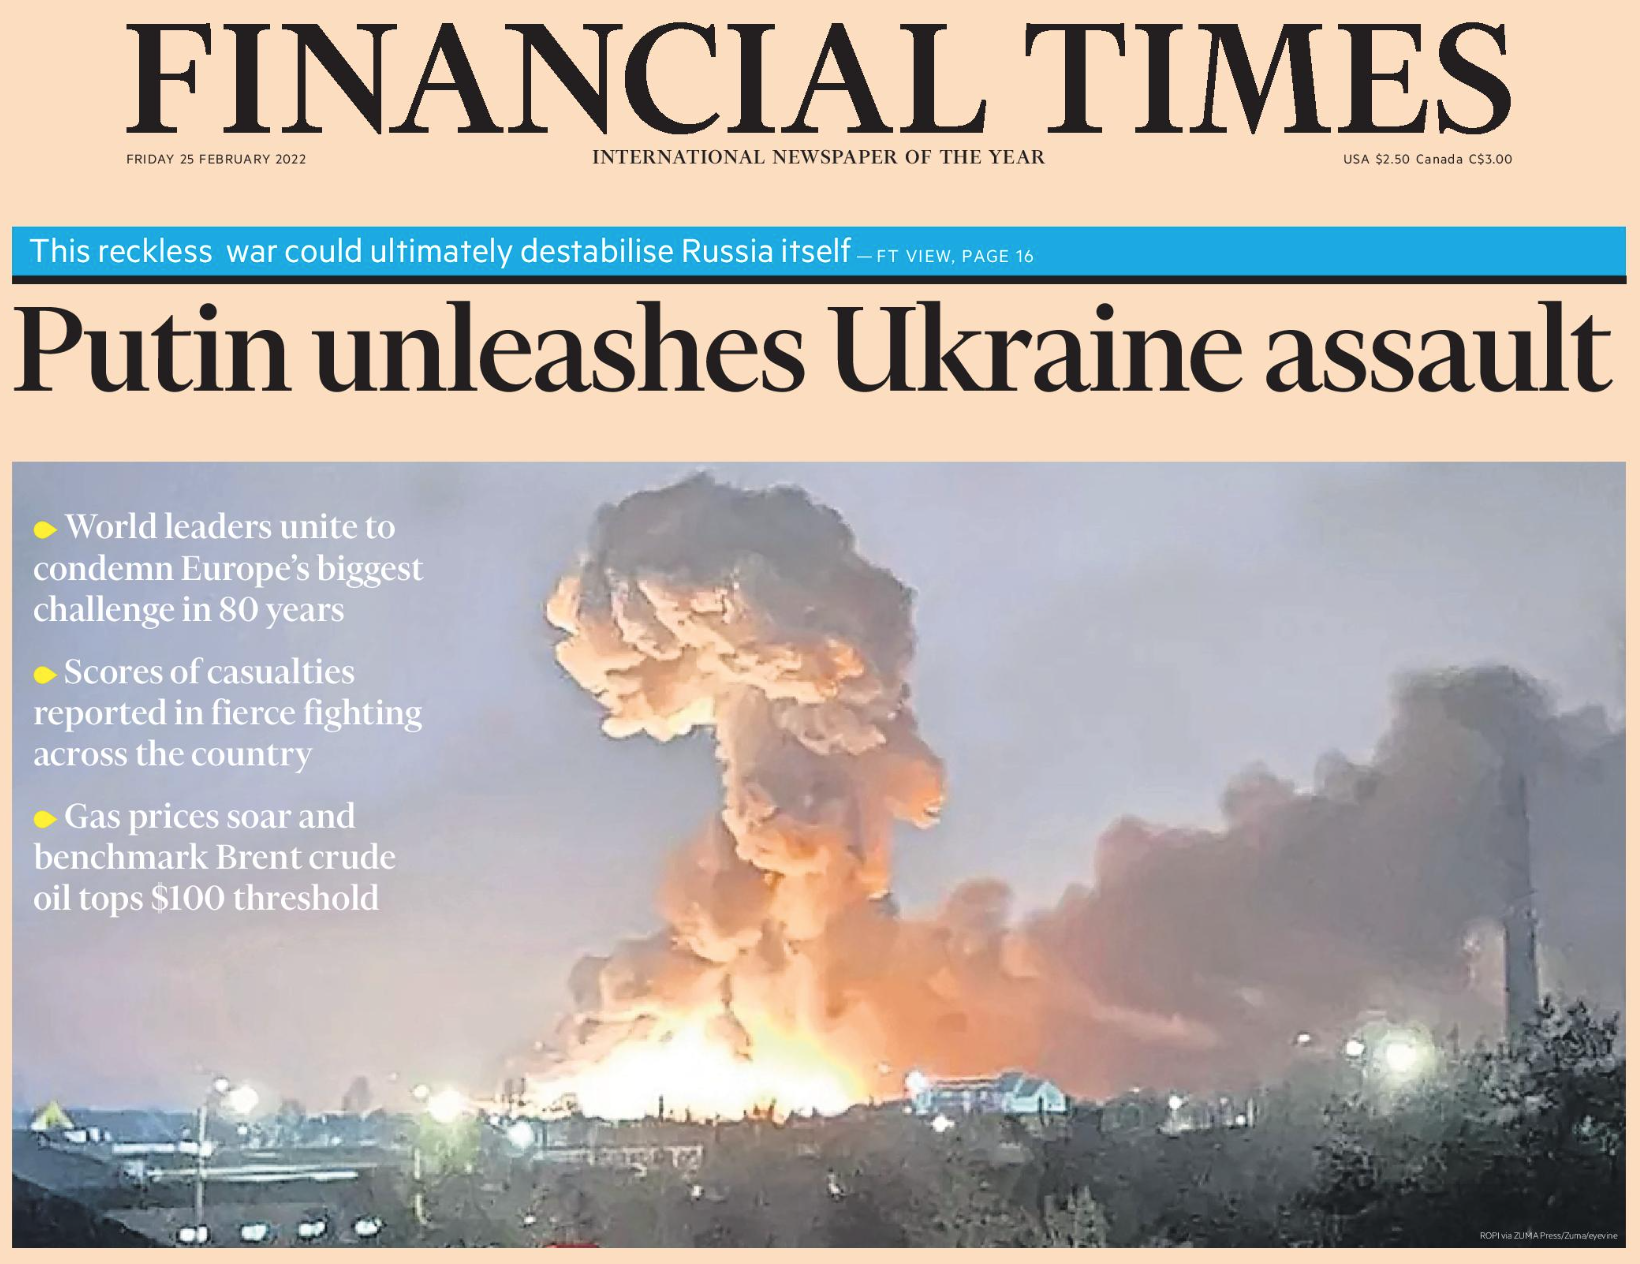
\includegraphics[width = 0.9\textwidth]{img/invasion_ft}

\end{frame}
% ----------------------------------------------------

\begin{frame}
\frametitle{Is this an inter-state war?}
\centering

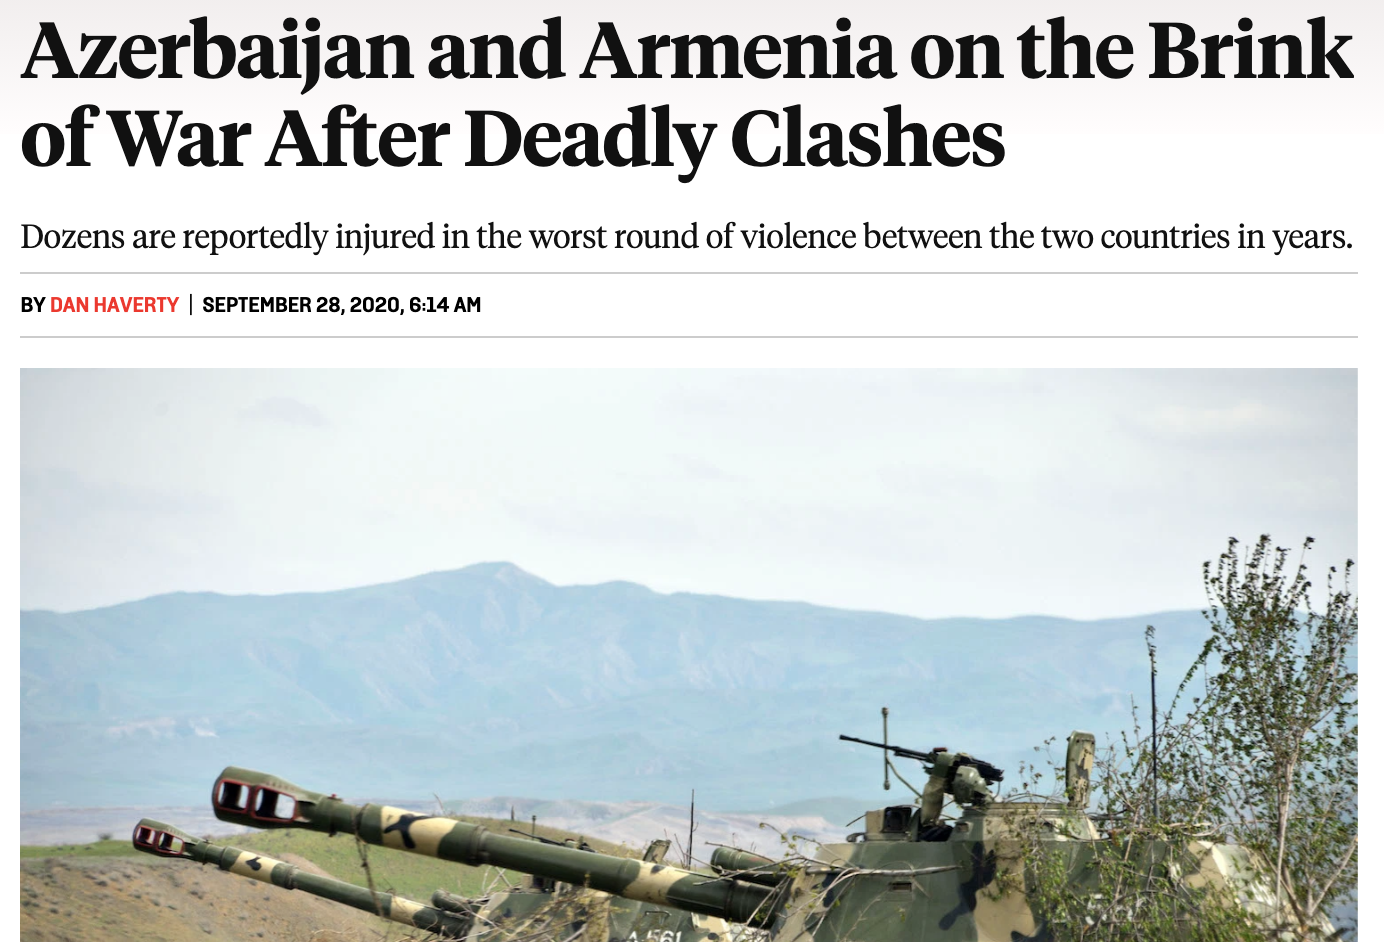
\includegraphics[width = 0.8\textwidth]{img/foreignaffairs_nagorno}

{\footnotesize \textit{FT,} September 2020.}

\end{frame}

\begin{frame}
\frametitle{Is this an inter-state war?}
\centering

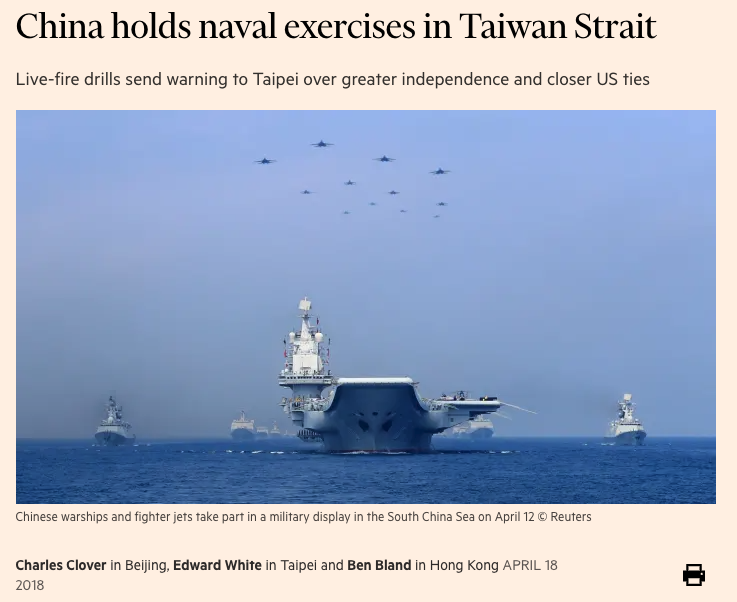
\includegraphics[width = 0.8\textwidth]{img/ft_south_china_sea}

{\footnotesize \textit{FT,} April 2018.}

\end{frame}

% ----------------------------------------------------
\begin{frame}
\frametitle{Why is important to distinguish wars from `non-wars'?}
\centering

\begin{itemize}
  \item Because we want to know how it relates to other situations, e.g.
  \begin{itemize}
    \item when do disputes escalate?
    \item when do civil wars lead to an interstate conflict?
    \item how frequent is unilateral aggression?
  \end{itemize}
  \item<2-> This has to do with the understanding of violence or aggression as a \textit{method} (not an end in itself) substituting for something else
\end{itemize}

\end{frame}
% ----------------------------------------------------

\begin{frame}
\frametitle{Inter-state wars}
\centering

\begin{itemize}
\item<1-> Sustained, military clash between two or more countries
  \begin{itemize}
  \item $\neq$ unilateral aggression, $\neq$ disputes
  \end{itemize}
\item<2-> How do we measure them?
\item<2->[] We usually employ intensity thresholds
  \begin{itemize}
  \item We want to separate wars from minor clashes or skirmishes (e.g. the Himalaya battles between China and India in 2020)
  \item A war can also be short: the Six-Day War (Israel \& Egypt) in 1967 killed +20,000
  \end{itemize}
\end{itemize}

\end{frame}


% ----------------------------------------------------
\imageframe{img/cow}
% ----------------------------------------------------

% ----------------------------------------------------
\begin{frame}
\frametitle{Measuring interstate war}
\centering

\begin{itemize}
  \item Coding wars in the Correlates of War project (\url{https://correlatesofwar.org/})
  \item ``sustained combat, involving organized armed forces, resulting in a minimum of 1,000 battle-related fatalities (later specified as 1,000 battle-related fatalities within a twelve month period)''
  \item Differentiating interstate wars from other types of wars (extra-state, intra-state, non-state)
\end{itemize}

\end{frame}
% ----------------------------------------------------

% ----------------------------------------------------
\begin{frame}
\frametitle{Correlates of War data project}
\centering

\begin{itemize}
  \item COW War Data, 1816 – 2007
  \item Militarized Interstate Disputes
  \item National Material Capabilities
  \item Militarized Interstate Dispute Locations
  \item Others
    \begin{itemize}
      \item Alliances, Contiguity, Territorial change, Defense Cooperation Agreement, etc
    \end{itemize}
\end{itemize}

\end{frame}
% ----------------------------------------------------

% ----------------------------------------------------
\begin{frame}
\frametitle{Understanding war}
\centering

\begin{itemize}[<+->]
  \item Why do wars break out?
  \item (We've seen the main IR theories, but neither they only cover wars nor wars are only explained by IR)
\end{itemize}

\end{frame}
% ----------------------------------------------------

% ----------------------------------------------------
\begin{frame}
\frametitle{Understanding war}
\centering

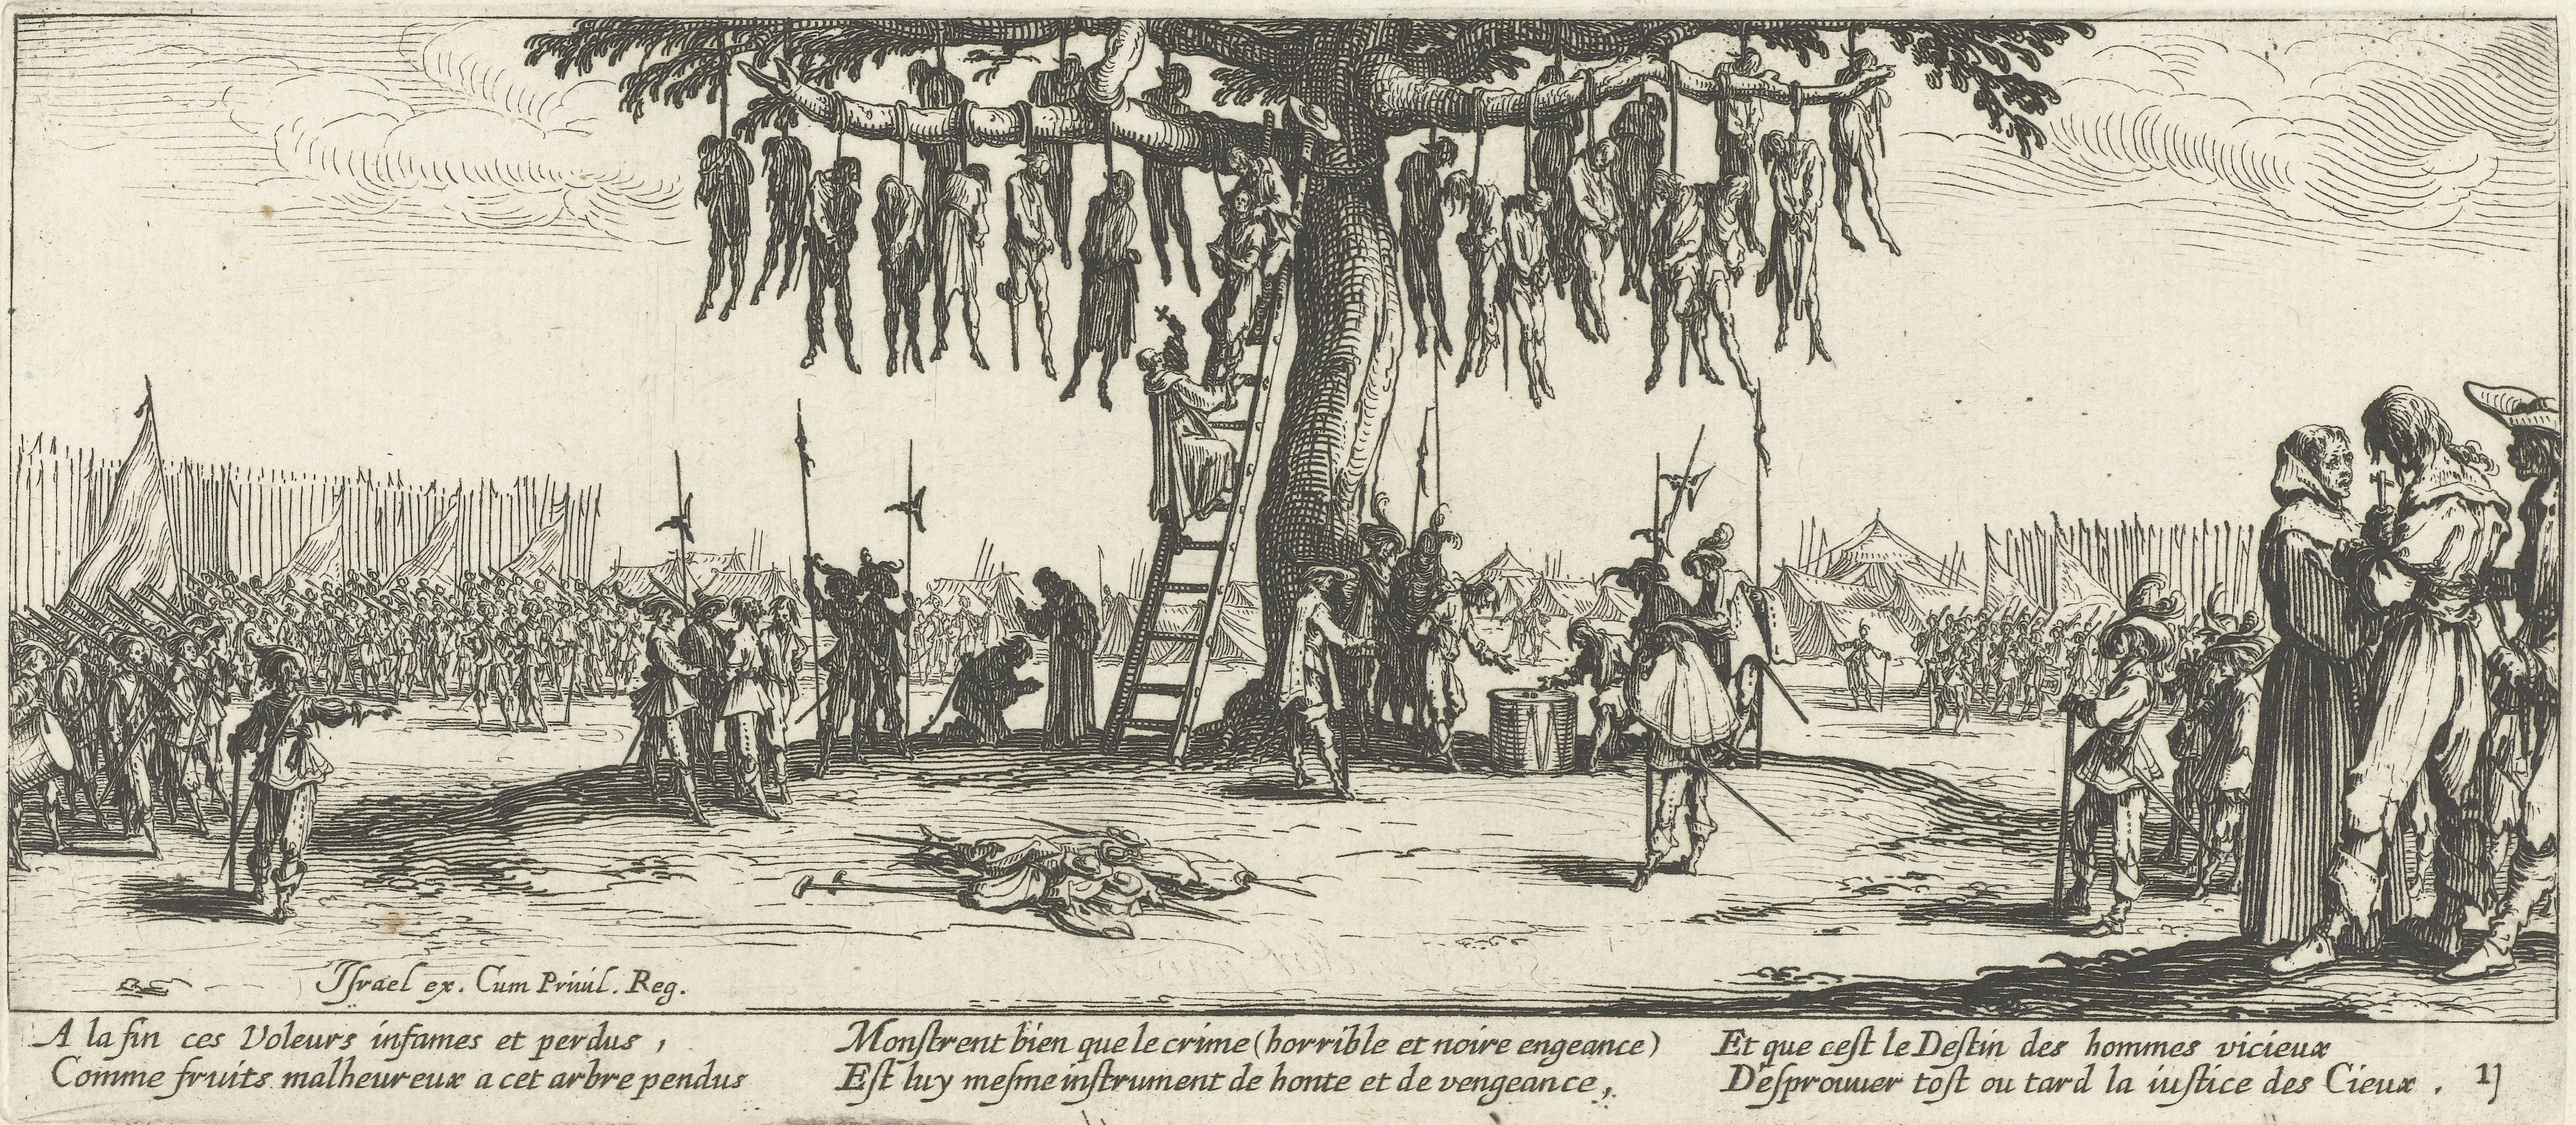
\includegraphics[width = 1\textwidth]{img/Jacques_Callot_hanging}

\vspace{15pt}

{\footnotesize Jacques Callot's \textit{Les Grandes Misères de la guerre} (1633)}


\end{frame}
% ----------------------------------------------------

\begin{frame}
\frametitle{Understanding war}
\centering

\uncover<1->{\begin{minipage}{0.66\textwidth}\centering
\begin{itemize}
\item<1-> ``War is the continuation of politics by other means''
\item<2-> Wars as a rational human phenomenon, against previous Enlightment view of war as a deviation
  \begin{itemize}
  \item Even in the 20th century, some still see it that way
  \end{itemize}
\item<2-> Part of the realist tradition: Thucydides, Machiavelli, Hobbes, etc
\end{itemize}
\end{minipage}}\hfill
\uncover<1->{\begin{minipage}{0.33\textwidth}\centering
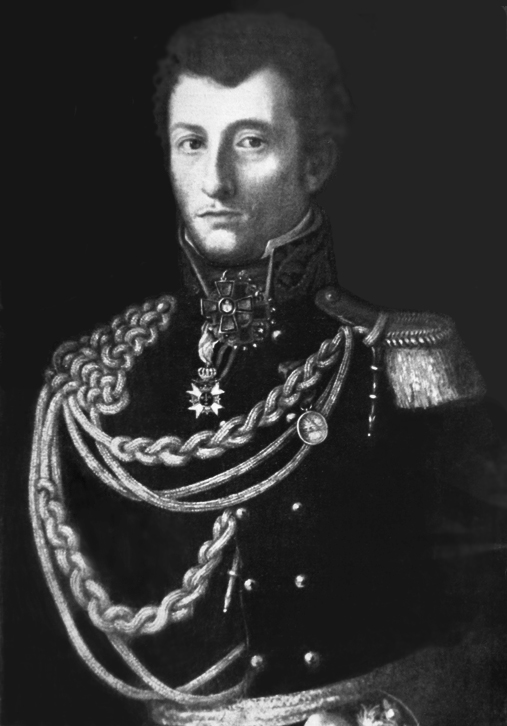
\includegraphics[width = 0.9\textwidth]{img/clausewitz}\\
Carl von Clausewitz\\{\small (\textit{On war}, 1832)}
\end{minipage}}

\end{frame}

\begin{frame}
\frametitle{Understanding war}
\centering

\begin{itemize}
\item Focus on the causes of war: why do wars break out?
\begin{itemize}
  \item[] ($\neq$ termination, consequences, conduct of war ...)
\end{itemize}
\item IR perspectives: realism, liberalism, constructivism
\item<2-> Main realist theories:
  \begin{itemize}
    \item \textbf{Balance of power works}: states pursue it internationally, (small) wars avoid larger ones, it deters aggression, etc
    \item<3-> \textbf{International hegemony}: no, alliances are actually war-prone -- given international anarchy, we need a Leviathan
    \item<3->[] (be careful when hegemony switches, though)
  \end{itemize}
\end{itemize}

\end{frame}

\begin{frame}
\frametitle{Liberal theories}
\centering

\begin{itemize}
  \item More popular explanations (nowadays), and also more geared to \textit{specific cases}
  \item Realist explanations are perhaps more focused on explaining system-wide instability
  \item Liberal theories are more applicable to specific states or dyads
  \begin{itemize}
    \item Even though they are also use to justify global systems
  \end{itemize}
  \item Two main theories:
  \begin{itemize}
    \item Democratic peace
    \item Capitalist peace
  \end{itemize}
\end{itemize}

\end{frame}


\begin{frame}
\frametitle{The democratic peace}
\centering

\begin{itemize}

\item<1-> When scholars began to collect statistics, found one law-like regularity: democracies do \textit{not} fight each other
  \begin{itemize}
  \item Kant already suggested it
  \end{itemize}
\item<2-> Even if the regularity exists, no agreement on the \textit{why}
  \begin{itemize}
  \item Democratic culture is more peaceful, democratic leaders are constrained by public opinion... (second image explanations)
  \item Common interests of democracies, historical learning process (system-level)
  \end{itemize}
\item<3-> Policy implications at the global and specific levels
\end{itemize}

\end{frame}

\begin{frame}
\frametitle{The capitalist peace}
\centering

\begin{itemize}
\item<1-> Main idea: `don't bite the hand that feeds you'
\begin{itemize}
  \item Related to 19th-century economic liberalism against mercantilism or nationalism: trade could improve the well-being of all countries, which also includes war
\end{itemize}
\item<2-> ``Opportunity cost'' hypothesis: if we benefit from trade, and war disrupts trade, the cost of fighting will be higher
  \begin{itemize}
  \item The more intense trade is, the most we will lose
  \item Domestic economic actors have incentives to influence
  \end{itemize}
\item<3-> Other theories point to the effects of economic prosperity
\item<3-> Some say that the democratic peace is not because democracy itself, but because of economic interdependences between wealthy countries (which happen to be democracies)
\end{itemize}

\end{frame}

% ----------------------------------------------------
\begin{frame}
\frametitle{Liberalism nowadays}
\centering

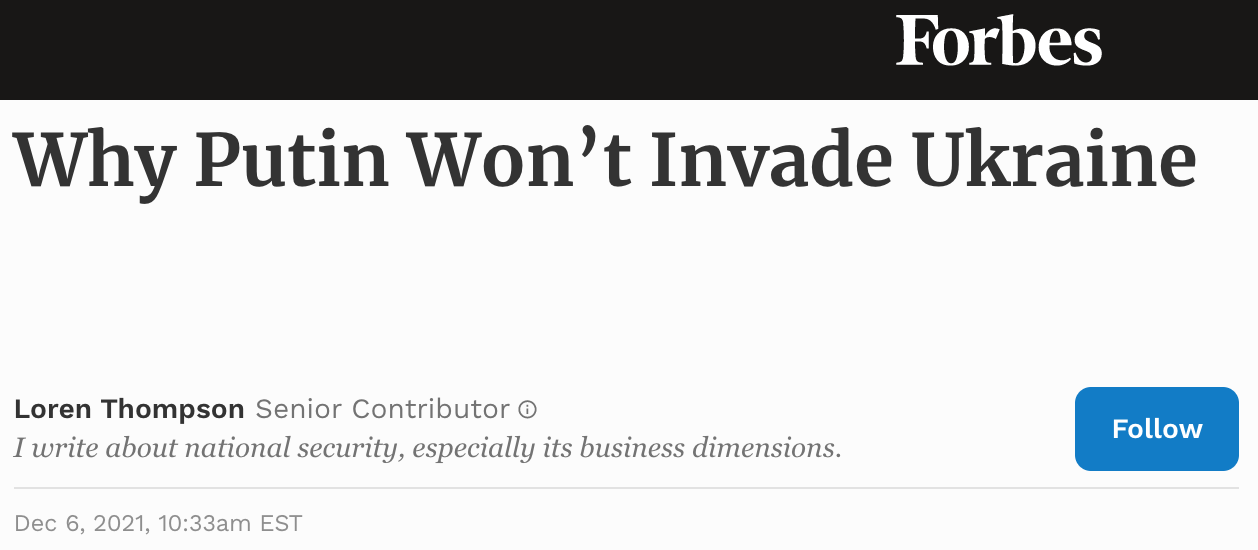
\includegraphics[width = 0.7\textwidth]{img/forbes_why_not1}\\
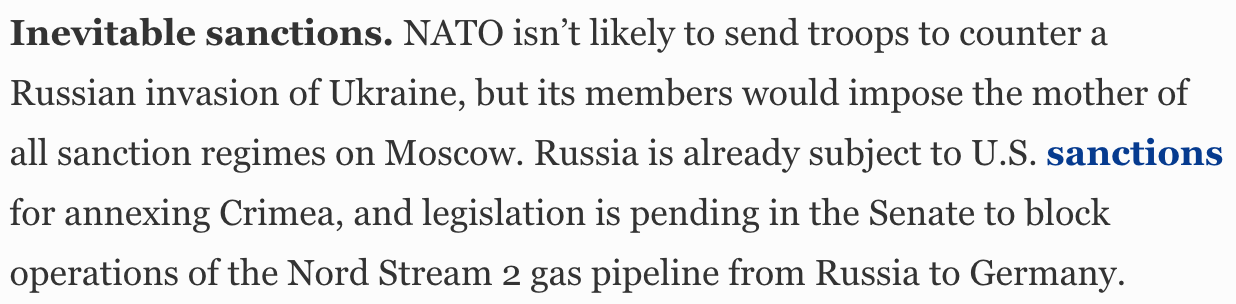
\includegraphics[width = 0.8\textwidth]{img/forbes_why_not2}\\
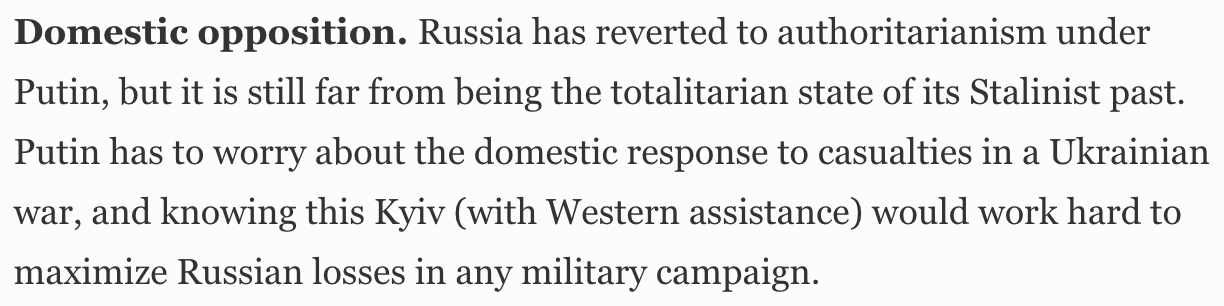
\includegraphics[width = 0.8\textwidth]{img/forbes_why_not3}

\end{frame}
% ----------------------------------------------------

\begin{frame}
\frametitle{Criticizing liberal theories}
\centering

\begin{itemize}
\item These theories have also been challenged, for example:
  \begin{itemize}
  \item Dyadic effects not taken into account: one side of the trading relationship could use war to increase their advantage
  \item Asymmetry can lead to exploitation (Marxists \& realists)
  \end{itemize}
\item Most empirical evidence suggests conflict-decreasing effect
\end{itemize}

\end{frame}


% ----------------------------------------------------
\begin{frame}
\frametitle{Constructivist theories}
\centering

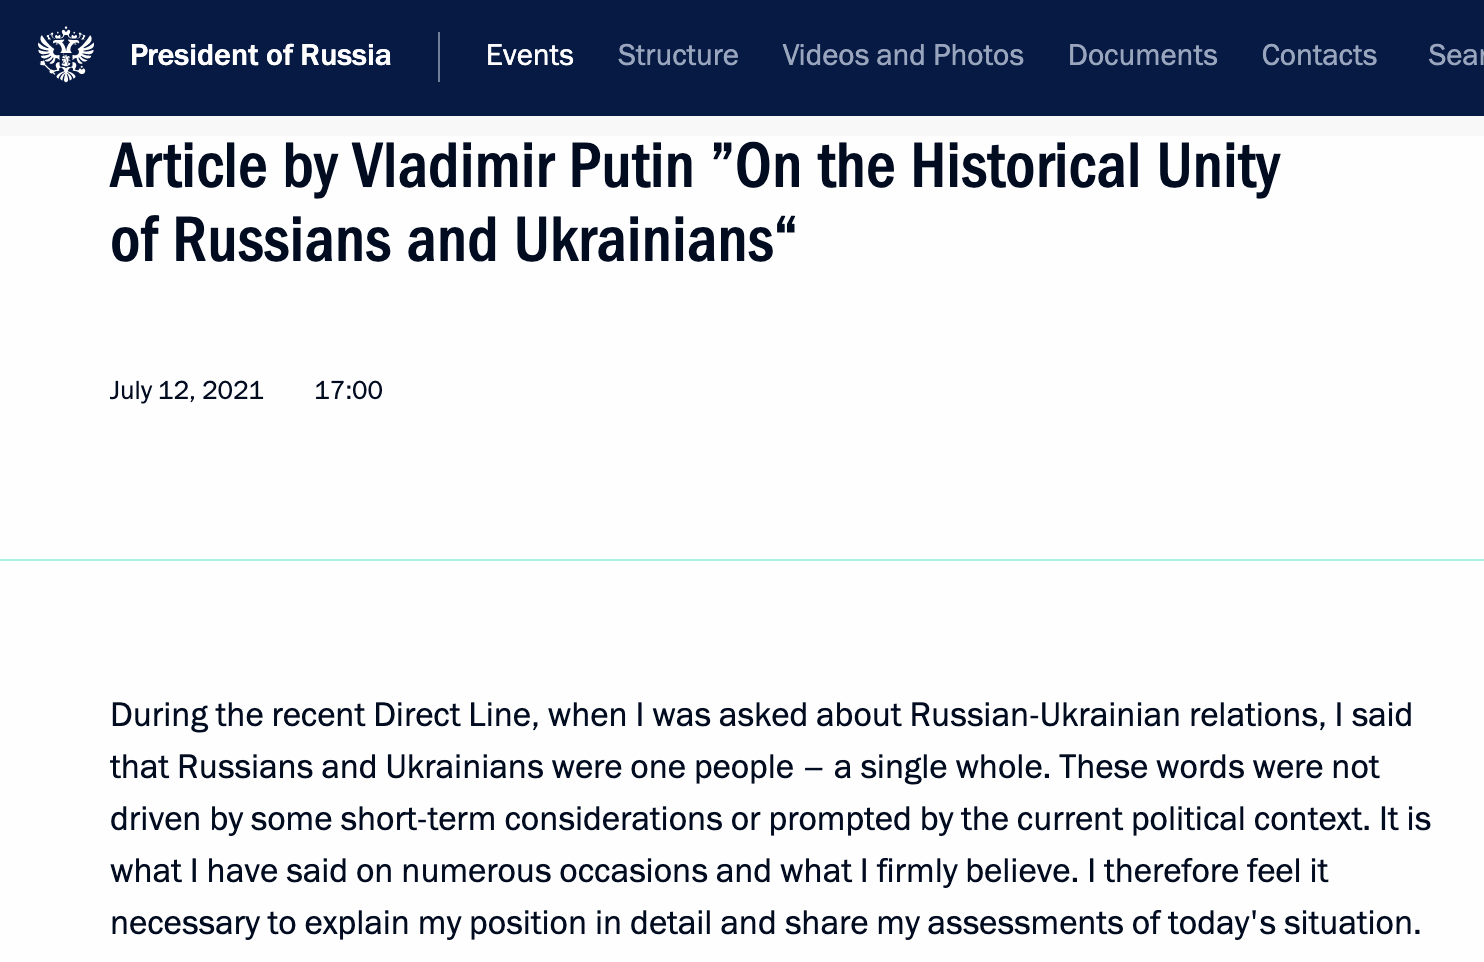
\includegraphics[width = 0.8\textwidth]{img/putin_historical_unity}

\begin{itemize}
  \item Also remember discussion from last day on ethnic groups
  \begin{itemize}
    \item probably more relevant in connection with other types of conflict
  \end{itemize}
\end{itemize}

\end{frame}
% ----------------------------------------------------

\begin{frame}
\frametitle{Rationalist theories of war}
\centering

\begin{itemize}
\item If we think of states as unitary rational actors, war is actually not rational, your theories do not have microfoundations
\end{itemize}

\vspace{15pt}

\uncover<2>{\footnotesize The \BGyellow{central puzzle about war}, and also the main reason we study it, is that \BGyellow{wars are costly but nonetheless wars recur}. Scholars have attempted to resolve the puzzle with three types of argument. \BGyellow{First}, \textbf{one can argue that people} (and state leaders in particular) \textbf{are sometimes or always irrational.} They are subject to biases and pathologies that lead them to neglect the costs of war or to misunderstand how their actions will produce it. \BGyellow{Second}, \textbf{one can argue that the leaders who order war enjoy its benefits but do not pay the costs}, which are suffered by soldiers and citizens. \BGyellow{Third}, \textbf{one can argue that even rational leaders} who consider the risks and costs of war may \textbf{end up fighting nonetheless.}}

\end{frame}

% ----------------------------------------------------
\imageframe{img/fearon_model}
% ----------------------------------------------------

\begin{frame}
\frametitle{Bargaining model of war}
\centering

  \begin{tikzpicture}[every text node part/.style={align=center}, scale = 0.75]

  % Process
  \node (a) at (0,0) {A};
  \node (b) at (10,0) {B};
  \draw[-] (a) -- (b);

  \uncover<2->{\draw (6, 0.2) -- (6, -0.2) node[below]{$p$};}
  \uncover<3->{\draw (4.5, 0.2) -- (4.5, -0.2) node[below]{\tiny $p-C_{a}$};}
  \uncover<3->{\draw (7.5, 0.2) -- (7.5, -0.2) node[below]{\tiny $p+C_{b}$};}
  \uncover<4->{\draw[->] (0, 1) -- (4.5, 1) node [above, midway] {\tiny A's expected gains};}
  \uncover<4->{\draw[<-] (7.5, 1) -- (10, 1) node [above, midway] {\tiny B's expected gains};}
  \uncover<5->{\draw[decorate,decoration={brace,amplitude=2pt}] (4.5, 2) -- (7.5, 2) node [above, midway, text width=2.3cm] {\tiny Bargaining space (anything here is better that fighting)\\};}

  \end{tikzpicture}

  \begin{itemize}
    \item<1> Imagine A and B are fighting over control of a territory, and A is a bit stronger than B (and both know this)
    \item<2> $p$ is what they expect if they fight
    \item<3-4> But war has a cost, so they would end up with a bit less
    \item<5> Therefore, under rational conditions, they would be better off if they negotiate before fighting
  \end{itemize}

\end{frame}

\begin{frame}
\frametitle{Bargaining model of war}
\centering

  \begin{tikzpicture}[every text node part/.style={align=center}, scale = 0.75]

  % Process
  \node (a) at (0,0) {A};
  \node (b) at (10,0) {B};
  \draw[-] (a) -- (b);

  \draw (6, 0.2) -- (6, -0.2) node[below]{$p$};
  \draw (4.5, 0.2) -- (4.5, -0.2) node[below]{\tiny $p-C_{a}$};
  \draw (7.5, 0.2) -- (7.5, -0.2) node[below]{\tiny $p+C_{b}$};
  \draw[->] (0, 1) -- (4.5, 1) node [above, midway] {\tiny A's expected gains};
  \draw[<-] (7.5, 1) -- (10, 1) node [above, midway] {\tiny B's expected gains};
  \draw[decorate,decoration={brace,amplitude=2pt}] (4.5, 2) -- (7.5, 2) node [above, midway, text width=2.3cm] {\tiny Bargaining space (anything here is better that fighting)\\};

  \end{tikzpicture}

% \vspace{55pt}

  \begin{itemize}
    \item[]
    \item This approach should be able to explain why there was never a \textbf{nuclear war}: the cost is just too high, even taking into account uncertainties
    \item[]
    \item[]
  \end{itemize}

\end{frame}


% ----------------------------------------------------
\begin{frame}
\frametitle{Bargaining model of war}
\centering

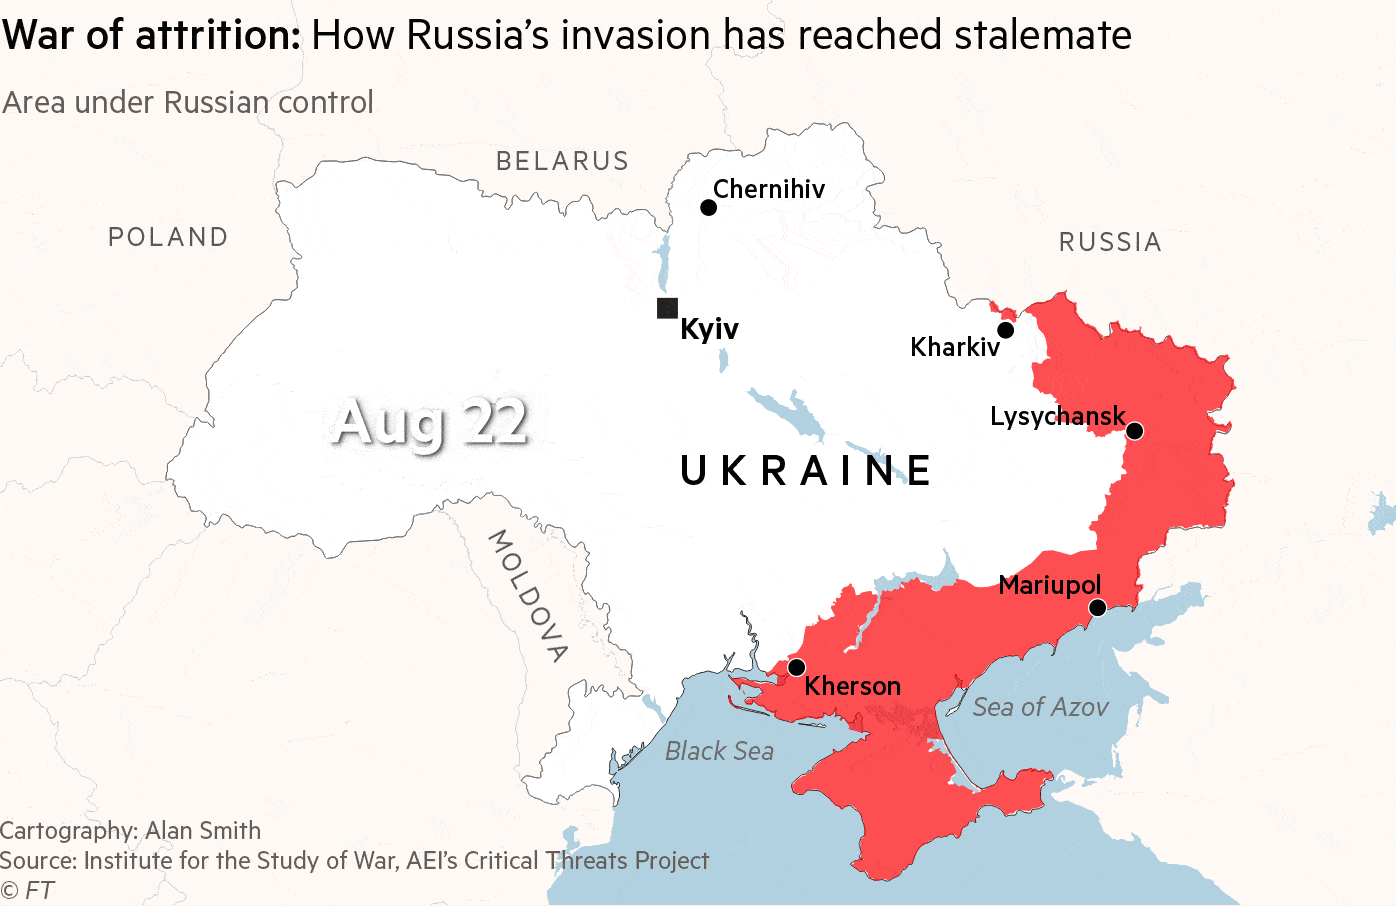
\includegraphics[width = \textwidth]{img/ft_ukraine_map}

\end{frame}
% ----------------------------------------------------

\begin{frame}
\frametitle{Rationalist theories of war}
\centering

\begin{itemize}
\item<1-> Why are states (or opposing parties) unable to reach a peaceful settlement before war? Three possibilities:
\item<2-> \BGyellow<2>{Private information}
  \begin{itemize}
  \item States do not have full information regarding the balance of power (like a Poker game, and war is like showing your cards)
  \end{itemize}
\item<3-> \BGyellow<3-4>{Commitment problems}
  \begin{itemize}
  \item When any kind of deal is unsustainable because of the incentive structure (e.g. Prisoner's dilemma), as when a declining powerful state has a dispute with an emerging new power
  \only<4>{\item Think about \textbf{preventive wars} or wars over bargaining issues that will affect \textbf{future balance of power}. Also, leaders could create or overcome them: sunk costs (e.g. mobilizing troops) or tying hands (e.g. domestic audiences)}
  \end{itemize}
\item<5-> \BGyellow<5>{Indivisible issues}
  \begin{itemize}
  \item If we are fighting for a piece of land or commercial rights, maybe we can split it up, but what if we are fighting for something sacred, e.g. control of Jerusalem? (constructivism!)
  \end{itemize}
\end{itemize}

\end{frame}

\begin{frame}
\frametitle{Two problems}
\centering

\begin{itemize}
\item<1-> Assumes that states are rational unitary actors, but what if they are not?
\item<2-> Within a state, there might be internal tensions (i.e. leaders are playing two games, one domestically and another one internationally)
  \begin{itemize}
  \item For instance, war could be beneficial to a leader that wants to avoid being seen capitulating
  \end{itemize}
\item<3-> Maybe rationality does not always apply
  \begin{itemize}
  \item Psychological biases, bounded rationality, etc
  \end{itemize}
\end{itemize}

\end{frame}

% \begin{frame}
% \frametitle{Psychological theories}
% \centering
%
% \begin{itemize}
% \item<1-> Modernized `first-image' account, focusing on two aspects of key decision-makers
% \item<2-> Their own psychology: belief systems, personalities, etc
%   \begin{itemize}
%   \item Formative experiences, education, culture...
%   \item Main idea: with a different leader, things would have gone differently
%   \end{itemize}
% \item<3-> Psychological processes involved in decision-making
%   \begin{itemize}
%   \item Bounded rationality: leaders are humans, and thus have limited capacities, limited access to information, cognitive biases, etc
%   \item Why people play the lottery? (Prospect theory \& Kahneman's \textit{Thinking, Fast and Slow}?)}
%   \end{itemize}
% \end{itemize}
%
% \end{frame}

\begin{frame}
\frametitle{Wraping up: what causes wars?}
\centering

\begin{itemize}[<+->]
\item This is just something very difficult to predict: `war is in the error term' (Gartzke)
\item A general theory of war is probably impossible: even if we account for system-level and state-level factors, individual characteristics and the decision-making process are hard to capture (especially empirically)
\item Also, some people say that the historical context matter when comparing wars
\end{itemize}

\end{frame}

\begin{frame}
\frametitle{Wraping up: what causes wars?}
\centering

\begin{itemize}
\item<1-> But we do know some empirical regularities over which new theories can be built, for example:
\item[]
\item[1.]<2-> Democracies and capitalist societies rarely fight each other
\item[2.]<3-> Many wars are fought among contiguous states over territorial disputes (which doesn't mean that neighbors usually fight each other)
\item[3.]<4-> Asymmetry does not usually lead to war, and wars are usually fought between strategic rivals
\end{itemize}

\end{frame}

% \begin{frame}
% \frametitle{Leaving out many other things}
% \centering
%
% \begin{itemize}
% \item Technology of warfare (regular and irregular wars)
% \item Historical evolution of technology and deterrence
% \item Conduct of war and wartime violence
% \item Consequences of inter-state war
% \item etc
% \end{itemize}
%
% \end{frame}

% \begin{itemize}
% \item Everything \textit{might} lead to war, nothing will \textit{certainly} lead to war
% \end{itemize}
%
% % Holsti, conclusions (as of 1991):
% % - single independent variables usually
% % - too many variables looked for
% % - most studies, only one level of analysis
% % (PUT TABLE in page 4?)
% >>> critique to ecological variables and their pitfalls etc
% >>> Holsti's approach:
% 1. importance of issues
% 2. historical context of war (can't compare a war in the 17th c with one in 1970)
% 3. link between peace settlements and future war
% >>> IR idea: beyond ecological factors, decision-making is important. Thucy's underlying and proximate causes of war.


% #### MORE TOPICS/SLIDES ####
% - TECHNOLOGY OF WAR (Boot's invisible armies? Check Laia & Kalyvas, who do they cite?)
% - IRREGULAR WARS (in inter-state war context! >> they are way more typical of civil war, why?)
% - EVOLUTION OF DAMAGE CAPACITY & DETERRENCE ERA
% - CONSEQUENCES OF INTER-STATE WAR (difference with legacies?): Morris (Tilly), Scheidel, Scheve & Stasavage

% \begin{frame}
% \frametitle{.}
% \centering
%
% Questions?
%
% \end{frame}


% ----------------------------------------------------
\begin{frame}
\frametitle{Interstate war in context}
\centering

\begin{tabular}{m{1.75cm}|m{4cm}m{4cm}}
& {\color{gray}{\footnotesize Target:}} \newline \BGasher<2,4>{State} & {\color{gray}{\footnotesize Target:}} \newline \BGasher<3,5>{Non-State} \\\hline\\
{\color{gray}{\footnotesize Perpetrator:}} \newline \BGasher<2-3>{State} & \BGyellow<2>{Interstate war} & \BGyellow<3>{State repression} \newline \BGyellow<3>{Genocide} \newline \BGyellow<3>{Ethnic cleansing} \\\\
{\color{gray}{\footnotesize Perpetrator:}} \newline \BGasher<4-5>{Non-State} & \BGyellow<4>{Mass protests (rebellion)} \newline \BGyellow<4>{Military coup} \newline \BGyellow<4>{Political assassination*} \newline \BGyellow<4>{Civil War} \newline \BGyellow<4>{Terrorism} \newline \BGyellow<4>{(Organized crime)} & \BGyellow<5>{Intercommunal violence*}\\\\\hline
\end{tabular}

\end{frame}
% ----------------------------------------------------

% ----------------------------------------------------
\begin{frame}
\frametitle{Connecting logics}
\centering

\begin{itemize}
  \item<1-> \textbf{Hierarchy}
  \begin{itemize}
    \item some types create the conditions for others to emerge within
    \item interstate wars can create genocides or revolutions
  \end{itemize}
  \item<2-> \textbf{Instrumentality}
  \begin{itemize}
    \item `using' a type of political violence as a tool to implement another
    \item terrorism can be used to win a civil war, or inter-communal violence to engage in a genocide
  \end{itemize}
  \item<3-> \textbf{Escalation}
  \begin{itemize}
    \item kind of like hierarchy, but in the opposite direction
    \item Syria 2011, 1936 coup in Spain, communal violence and civil war?
  \end{itemize}
  \item<4-> \textbf{Substitution}
  \begin{itemize}
    \item strategic choice between two types of civil wars
    \item proxy wars during the Cold War, terrorists and civil wars, genocide and ethnic cleansing (Plan Madagascar)
  \end{itemize}
\end{itemize}

\end{frame}
% ----------------------------------------------------

% ----------------------------------------------------
\begin{frame}
\frametitle{Friday seminar}
\centering

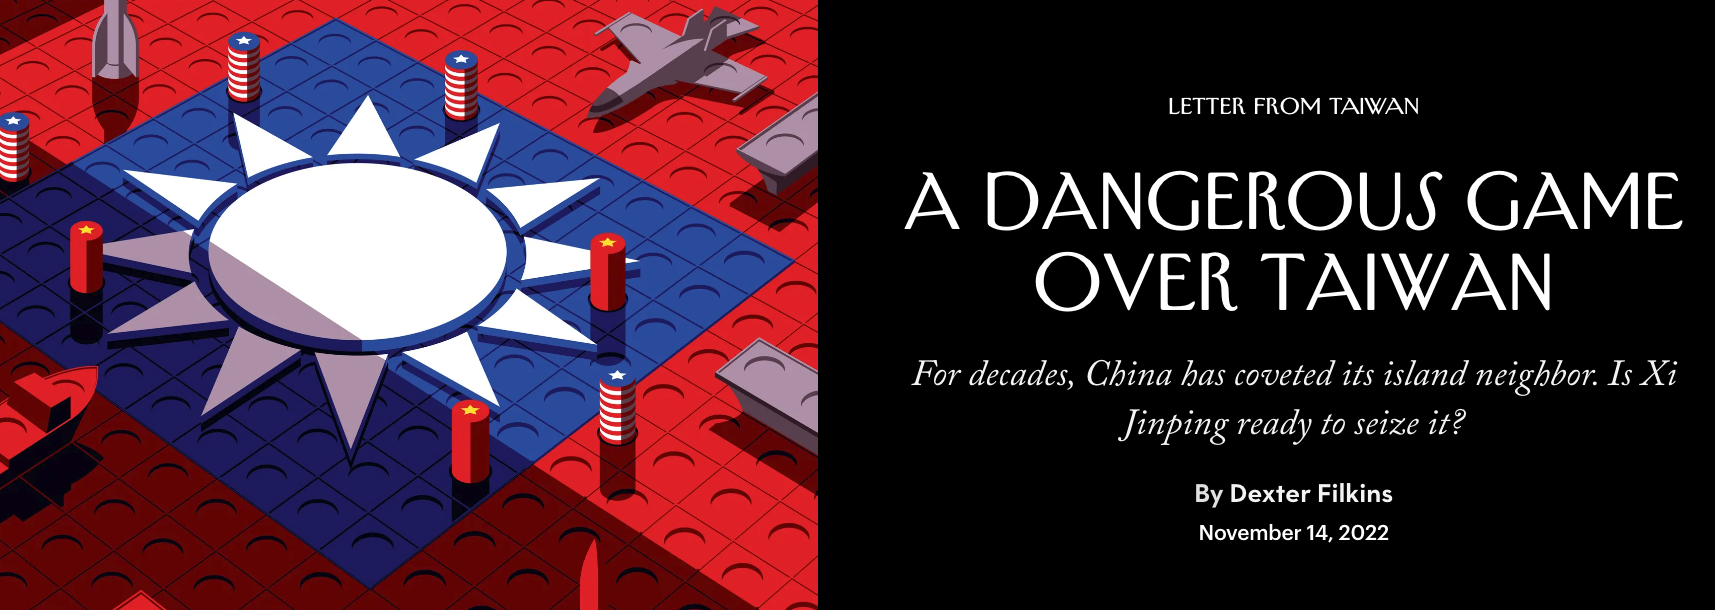
\includegraphics[width = \textwidth]{img/ny_taiwan}

\end{frame}
% ----------------------------------------------------

% ----------------------------------------------------
\begin{frame}
\frametitle{Exam question from Dec 2022}
\centering

\begin{itemize}
  \item Tensions between China and the US have increased significantly during the last few months, related to the conflict over Taiwan. As a result, there has been some discussion lately about the risk of a potential open conflict between the US and China in the near future (\href{https://www.newyorker.com/magazine/2022/11/21/a-dangerous-game-over-taiwan}{e.g.}). Yet, \textit{beyond} a US-China war, how do you think this increase in tensions and the growing (military) power of China can affect patterns of political violence across the world? (1000 words)
\end{itemize}

\end{frame}
% ----------------------------------------------------

\end{document}
